\documentclass{standalone}
\usepackage{tikz}

\begin{document}

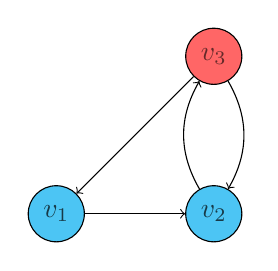
\begin{tikzpicture}
    \node[shape=circle,draw=black, fill=cyan, fill opacity=0.7] (v1) at (0,0) {$v_1$};
    \node[shape=circle,draw=black, fill=cyan, fill opacity=0.7] (v2) at (2,0) {$v_2$};
    \node[shape=circle,draw=black, fill=red, fill opacity=0.6] (v3) at (2,2) {$v_3$};

    \path [->] (v1) edge node[left] {} (v2);
    \draw[->] (v2) to[out=120,in=240] (v3);
    \draw[->] (v3) to[out=300,in=60] (v2);
    \path [->] (v3) edge node[left] {} (v1);  

\end{tikzpicture}

\end{document}